\subsection*{Náhodnost (background)}

\begin{defn}[Probabilistic TM]
	Probabilistic TM is a NTDM with a function $P:(Q\times \Sigma \times Q \times \Sigma \times M)\rightarrow [0,1]$ s.t.
	\[
		\forall (q,a) \in Q\times \Sigma: \Sigma_{(q',\sigma',m') \in Q\times \Sigma \times M}P(q,\sigma,q',\sigma',m)=1,
	\]
	$Q$ being a set of possible states and $M=\{\leftarrow\,\rightarrow,\_\}$.
\end{defn}

\begin{defn}[Zanedbatelná funkce]
	$\mu:\N\mapsto\R_+$ je zanedbatelná, jestliže pro každý polynom $p$ existuje $n_p \in \N$ takové, že
	\[
		\forall n \geq n_p: \mu(n)\leq\frac{1}{p(n)}.
	\]
\end{defn}

V této části nás budou zajímat především soubory náhodných veličin $\{X_i\}_{i\in\N}$, $X_i$ nabývá hodnot z $\{0,1\}^{l(i)}$ pro $l(i):\N\mapsto \N$. Obvykle $l(i)\geq i$, nicméně často budeme uvažovat $l(i)=i$. Pro tyto soubory se budeme snažit zjistit podobnost se soubory $\{U_n\}_{n\in\N}$ příslušných rovnoměrně rozdělených náhodných veličin.

\begin{defn}[Blízkost souborů]
	Buďtež $\{X_i\}_{i\in\N}$ a $\{Y_i\}_{i\in\N}$ dva soubory náhodných veličin. Pak rozlišujeme tyto stupně blízkosti souborů náhodných veličin:
	\begin{itemize}
		\item Soubory jsou identické, pokud pro všechna $n\in\N$ platí $X_n=Y_n$, tj. $X_n$ a $Y_n$ mají stejné rozdělení.
		\item Soubory jsou \textit{statisticky blízké}, jestliže jejich \textit{statistická diference} $\Delta_{X,Y}(n)$ je zanedbatelná funkce.
		\[
			\Delta_{X,Y}(n) = \frac{1}{2}\Sigma_{v\in\{0,1\}^n}|Pr[X_n=v]-Pr[Y_n=v]|
		\]
		\item Soubory jsou \textit{výpočetně nerozlišitelné}, jestliže pro každý polynomiální pravděpodobnostní algoritmus $D$ je $\delta_{D,X,Y}(n)$ zanedbatelná funkce.
		\[
			\delta_{D,X,Y}(n) = |Pr[D(X_n)=1]-Pr[D(Y_n)=1]|
		\]
		\item Soubory jsou \textit{silně výpočetně nerozlišitelné}, jestliže pro každý soubor obvodů $\mathcal{C}=\{C_n\}_{n\in\N}$ polynomiální velikosti je $\sigma_{\mathcal{C},X,Y}(n)$ zanedbatelná funkce.
		\[
			\delta_{D,X,Y}(n) = |Pr[C_n(X_n)=1]-Pr[C_n(Y_n)=1]|
		\]
	\end{itemize}
\end{defn}

\begin{defn}
	Řekneme, že soubor náhodných veličin $\{X_i\}_{i\in\N}$ je \textit{(silně) pseudonáhodný}, jestliže je (silně) výpočetně nerozlišitelný od souboru $\{U_n\}_{n\in\N}$ náhodných veličin s uniformním rozdělením.
\end{defn}

\begin{defn}[jednosměrná funkce]
	Funkce $F:\{0,1\}^*\mapsto \{0,1\}^*$ je jednosměrná, jestliže je spočitatelná v polynomiálním čase a je těžko invertovatelná, tj. pro každý pravděpodobnostní polynomiální algoritmus $B$ je funkce
	\[
		Pr_{x\sim U_n}[B(f(x)) \in f^{-1}\circ f(x)],\ x\sim U_n
	\]
	zanedbatelná v $n$.
\end{defn}

Zvláštním případem jsou \textit{jednosměrné permutace}, prosté jednosměrné funkce zachovávající délku vstupu.

\begin{defn}[Těžký bit]
	Zobrazení $b:\{0,1\}^*\mapsto \{0,1\}$ je \textit{těžký bit} funkce $f$, jestliže platí:
	\begin{itemize}
		\item $b$ je spočitatelné v polynomiálním čase
		\item není odhadnutelné s nezanedbatelnou výhodou, tj. pro každý pravděpodobnostní algoritmus $B$ je funkce
		\[
			|Pr_{x\sim U_n}[B(f(x)) = b(x)]-\frac{1}{2}|
		\]
		zanedbatelná v $n$.
	\end{itemize}
\end{defn}

Je-li $f$ prostá, pak má těžký bit, právě když je jednosměrná. V opačném případě bychom mohli hodnotu bitu $b(x)$ spočíst invertováním $f(x)$. Pokud by naopak bylo možné s nezanedbatelnou pravděpodobností spočíst libovolný bit $x_i$, pak bychom mohli vzor spočíst s nezanedbatelnou pravděpodobností i celé $x$.

Pro neprosté funkce je situace složitější, jelikož požadujeme nalezení právě použitého $x$, nikoliv jiného se stejným obrazem. Pak tedy například $f(x)$ má dva stejně pravděpodobné vzory $x$ a $x'$ a $b(x)\neq b(x')$, pak je odhad nemožný.

\begin{lemma}\label{lemma:oracle}
	Pro $x$ délky $n$ označme $b_x(r)$ orákulum splňující
	\[
		|Pr_{r\sim U_n}[b_x(r)=\langle x,r\rangle]-\frac{1}{2}| \geq \varepsilon(n).
	\]
	Existuje pravděpodobnostní algoritmus $A$ pracující v čase polynomiálním čase v $(\frac{n}{\varepsilon(n)})$ takový, že pro každé $x$ platí
	\[
		Pr[A^{b_x}(1^n)=x]\geq \frac{\varepsilon(n)^2}{2n}.
	\]
\end{lemma}

\begin{thm}
	Nechť $f$ je libovolná jednosměrná funkce. Definujme funkci $g$ předpisem
	\[
		g(x,r):=(f(x),\,r), |x|=|r|. 
	\]
	Pak bodový součin vektorů $x,\,r$ modulo $2$ je těžkým bitem funkce $g$.
	\begin{proof}
		Nechť $\langle x,r \rangle$ není těžký bit funkce $g$ a označme $G$ algoritmus, který to dokazuje a označme $\gamma$ jeho výhodu:
		\[
			\gamma(n)=|Pr_{x,r\sim U_n}[G(f(x),r) = \langle x,r\rangle]-\frac{1}{2}|.
		\]
		Budiž $S_n$ množina takových $x$ délky $n$, na kterých je výhoda $G$ alespoň $\gamma(n)/2$. Tato množina má velikost alespoň $\frac{\gamma(n)}{2}2^n$, jinak by výhoda $G$ byla menší než
		\[
			\frac{1}{2^n}\left(\Sigma_{x\in S_n}1+\Sigma_{x\not\in S_n}\frac{\gamma(n)}{2}\right)<\frac{\gamma(n)}{2}+\frac{\gamma(n)}{2}=\gamma(n)
		\]
		Dle Lemmatu \ref{lemma:oracle} lze pro každé $x\in S_n$ v čase, který je polynomiální v $n/\gamma(n)$ a s pravděpodobností alespoň poly($\gamma(n)/n$) najít $x$ s pomocí $f(x)$ ($b_x(r)=G(f(x),r)$). Protože $x\sim U_n$ leží v $S_n$ s pravděpodobností alespoň $\gamma(n)/2$ a $\gamma(n)$ není zanedbatelná, dostáváme spor s jednosměrností $f$.
	\end{proof}
\end{thm}

Buď $f$ jednosměrná funkce a $b$ její těžký bit, pak závazkem může být $Z(m,x):=(f(x),m\oplus b(x))$, autorizací k otevření závazku je $x$.

\subsection*{Generátory pseudonáhodných čísel}

\begin{defn}
	(Neuniformně silný) pseudonáhodný generátor je deterministický algoritmus $G$, který vstup délky $n$ prodlužuje na výstup délky $l(n)>n$ tak, že soubor $\{G(U_n)\}_{n\in N}$ je (silně) pseudonáhodný.
\end{defn}

\begin{thm}
	Nechť je $f$ jednosměrná permutace a b její těžký bit. Pak je zobrazení $G:x\mapsto f(x)\parallel b(x)$ pseudonáhodný generátor.
	\begin{proof}
		Chceme rozlišit $f(x)\parallel b(x)$ od náhodné posloupnosti, tzn. chceme uhodnout $b(x)$ z $f(x)$.

		Nechť $G$ není pseudonáhodný generátor a $D$ je algoritmus, který to dokazuje, tj. $|Pr[D(f(x)b(x))=1]-Pr[D(y')=1]|=\varepsilon(n)$, $\varepsilon$ nezanedbatelná funkce. Toto lze přepsat do formy
		\[
			|Pr[D(y\parallel b\circ f^{-1}(y))=1]-Pr[D(y\parallel \sigma)=1]|=\varepsilon(n).
		\]
		Protože s pravděpodobností $1/2$ platí $\sigma=b\circ f^{-1}(y)$, pak také
		\[
			Pr[D(y\parallel\sigma)=1]=\frac{1}{2}Pr[D(y\parallel b\circ f^{-1}y)=1]+\frac{1}{2}Pr[D(y\parallel \overline{b\circ f^{-1}y})=1]
		\]
		\[
			|Pr[D(y\parallel b\circ f^{-1}y)=1]-Pr[D(y\parallel \overline{b\circ f^{-1}y})=1]|=2\varepsilon(n)
		\]
		Rozlišovač $A(y):=\sigma$, jestliže $D(y\parallel\sigma)=1$, $A(y):=\overline{\sigma}$ v opačném případě. Úspěšnost $A$ je:
		\[
			Pr[A(y)=b\circ f^{-1}(y)]=
		\]
		\[
			=Pr[D(y\parallel\sigma)=1 \land \sigma=b\circ f^{-1}(y)]+Pr[D(y\parallel\sigma)=0 \land \overline{\sigma}=b\circ f^{-1}(y)]
		\]
		\[
			\frac{1}{2}Pr[D(y\parallel b\circ f^{-1}(y))=1]+\frac{1}{2}Pr[D(y\parallel \overline{b\circ f^{-1}(y)})=0]
		\]
		\[
			\frac{1}{2}Pr[D(y\parallel b\circ f^{-1}(y))=1]+\frac{1}{2}(1-Pr[D(y\parallel \overline{b\circ f^{-1}(y)})=1])
		\]
		\[
			\frac{1}{2}+\frac{1}{2}(Pr[D(y\parallel b\circ f^{-1}(y))=1]-Pr[D(y\parallel \overline{b\circ f^{-1}(y)})=1])=\frac{1}{2}\pm\varepsilon(n)
		\]
		Výhoda $A$, tj. $|Pr[A(y)=b\circ f^{-1}(y)]-\frac{1}{2}|$, není zanedbatelná funkce, což je spor s předpokladem, že $b$ je těžký bit.
	\end{proof}
\end{thm}

\begin{thm}
	Nechť G je pseudonáhodný generátor s prodlužovací funkcí $l(n)=n+1$ a nechť $l'$ je libovolný polynom. Definujme zobrazení $G'$ předpisem
	\[
		G'(s)=\sigma_1(s)\parallel\dots\parallel\sigma_{l'(|x|)}(s),
	\]
	kde
	\[
		x_0=s,\ G(x_{i-1})=x_i\parallel\sigma_i(s),\, i=1,2,\dots,l'(|x|).
	\]
	Pak je $G'$ pseudonáhodný generátor.
	\begin{proof}
		Buď $X_1,\dots,X_{l'(n)}$ nezávislé kopie náhodné proměnné $U_1$. Budeme chtít ukázat, že $(X_1,\dots)$ neumíme rozlišit od $(\sigma_1(s),\dots)$ s nezanedbatelnou výhodou. Zdůrazněme, že $\sigma_i(s)$ vycházejí ze stejné volby $s$ a jsou tedy závislé. Zadefinujme si hybridní distribuci:
		\[
			H^{(i)}=(X_1,\dots,X_i,\sigma_1(s),\dots,\sigma_{l'(n)-i}(s))
		\]
		Algoritmus $D$, který rozlišuje $H^{(0)}$ od $H^{l'(n)}$ s nezanedbatelnou výhodou, rozlišuje taktéž s nezanedbatelnou výhodou nějaké $H^{(i)}$ od $H^{(i+1)}$. Předpokládejme, že jsme takové $i$ zvolili ($Pr=1/l'(n)$). Pro dané $y\parallel\sigma$ necháme rozhodnout
		\[
			(X_1,\dots,X_i,\sigma,\sigma_1(y),\dots,\sigma_{l'(n)-i-1}(y))
		\]
		Je-li $y\parallel\sigma\sim U_{n+1}$, jde o $H^{(i+1)}$. Je-li $y\parallel\sigma=G(s)$ pro $s \sim U_n$, jde o $H^{(i)}$, protože $\sigma=\sigma_1(s)$ a $\sigma_i(y)=\sigma_{i+1}(s)$.
	\end{proof}
\end{thm}

\subsection*{Důkazy s nulovou znalostí}
\begin{defn}[ITM]
	\textit{Interaktivní Turingův stroj} je vícepáskový pravděpodobnostní TM se vstupem a výstupem, který kromě vstupní pásky (\textit{veřejná}), výstupní pásky a pracovní pásky obsahuje ještě
	\begin{itemize}
		\item dodatečnou vstupní pásku (\textit{soukromá})
		\item \textit{vstupní komunikační pásku} (read-only)
		\item \textit{výstupní komunikační pásku} (write-only)
		\item \textit{stavový bit} (1 políčko s 1/0)
	\end{itemize}
	Stroji je přiřazena \textit{identita} jedna nebo 0. Program pak obsahuje instrukce pouze pro případ, že je stavový bit roven identitě stroje. V takovém případě stroj pracuje, jinak je \textit{nečinný}.
\end{defn}

\begin{defn}\label{def:is}
	\textit{Interaktivní systém} je dvojice ITM $(A,B)$, které
	\begin{itemize}
		\item mají opačnou identitu,
		\item sdílí veřejnou vstupní pásku,
		\item sdílejí stavový bit,
		\item vstupní komunikační páska $A$ je výstupní komunikační páskou $B$ a naopak.
	\end{itemize}
	Konvence: $A$ \textit{dokazovatel}, $B$ \textit{ověřovatel}; tj. výstupem interaktivního výpočtu je pouze výstup $B$ a složitost se bere v potaz pouze u ověrovatele.
\end{defn}

\begin{defn}[IP]
	$L \in IP \Leftrightarrow \exists$ interaktivní systém $(A,B)$ t.ž.
	\begin{itemize}
		\item (efficiency) poly-time
		\item (completeness) $(A,B)$ přijme $x\in L$ s pr. alespoň $2/3$
		\item (soundness) $x\not\in L$, pak pro lib. ITM $A^*$ je pravděpodobnost, že $(A^*,B)$ přijme $x$, menší než $1/3$.
	\end{itemize}
\end{defn}

\begin{thm}
	\begin{enumerate}
		\item $BPP \subseteq IP$
		\item $NP \subseteq IP$
	\end{enumerate}
	\begin{proof}
		1: $L\in BPP$ a $B$ ho rozhoduje ve smyslu $BPP$. Pak $(\emptyset,B)$ rozhoduje $L$ ve smyslu $IP$ -- výpočet proběhne v jedné fázi.

		2: $L\in NP$, $A$ sdělí slovo $y$ (svědek $x$) $B$. $B$ ověří, že $y$ je ve svědecké relaci s $x$ (ověření v poly-time, úplnost daná existencí svědka, spolehlivost z neexistence svědka pro $x\not\in L$)
	\end{proof}
\end{thm}
\pagebreak
\begin{defn}[Grafový neisomorfismus]
	GraphNI=$\{(G_1,G_2)|G_1\not\cong G_2\}$
\end{defn}

Grafový neizomorfismus je zřejmě v $PSPACE$ (mohu in-place vyzkoušet všechna řešení).

\begin{claim}
	$GraphNI \in IP$
	\begin{proof}
		Uvažme dvě kola uvedené komunikace. Efektivita je zřejmá. Pokud $(G_0,G_1) \in GraphNI$, pokud $\varphi(H)=G_j$, pak platí $i=j$ -- $B$ přijme vstup s pravděpodobností 1 (úplnost).

		$(G_0,G_1)\not\in GraphNI$, tj. grafy jsou izomorfní. Definujme multiset
		\[
			M_i:=\{\pi(G_i)|\pi\in S_n\},\ i=0,1.
		\]
		Zřejmě v tomto případě $M_0=M_1$, tj. $A$ odpoví nezávisle na volbě $i$. Z uniformity volby $i$ je tedy pr. přijetí vstupu $(\frac{1}{2})^2$, čímž je dokázána spolehlivost.

		\begin{figure}[H]
			\centering
			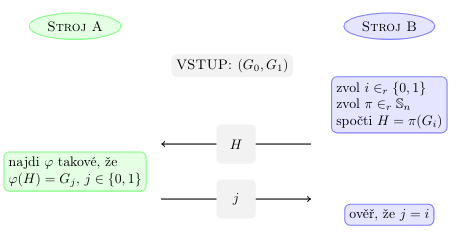
\includegraphics[width=0.5\linewidth]{graph_niso}
		\end{figure}
	\end{proof}
\end{claim}

\begin{thm}[Shamir]
	$IP = PSPACE$
\end{thm}

\begin{defn}
	Interaktivní důkazový systém $(A,B)$ se nazývá \textit{důkaz s nulovou znalostí} (zero-knowledge proof) pro jazyk $L$, pokud rozhoduje jazyk ve $L$ ve smyslu Definice \ref{def:is} a navíc pro každý interaktivní stroj $B^*$ existuje poly-time PTM $M$ takový, že pro každé $x\in L$ platí:
	\begin{itemize}
		\item $Pr[M(x)=\perp]\leq 1/2$ (výpočet $M$ selhal)
		\item $M(x)\neq\perp\Rightarrow M(x)\sim \sigma_F(A,B^*)(x)$ pro $\sigma_F(A,B^*)(x)$ závěrečný snímek $B*$ po výpočtu $(A,B^*)$ na $x$.
	\end{itemize}
	Symbol $\sim$ odpovídá jednomu ze stupňů blízkosti ($\{M(x)\}_{x\in L}$ i $\{\sigma_F(A,B^*)(x)\}_{x\in L}$ soubory náhodných veličin):
	\begin{itemize}
		\item $\sim$ rovnost souborů -- \textit{důkaz s dokonale nulovou znalostí} (třída PZK),
		\item $\sim$ statistická blízkost -- \textit{důkaz s téměř dokonalou nulovou znalosti} (třída SZK),
		\item $\sim$ výpočetní nerozlišitelnost -- \textit{důkaz s výpočetně nulovou znalosti} (třída CZK).
	\end{itemize}
\end{defn}

Poznamenejme, že $M$ neumí rozhodovat jazyk -- simulátor je úspěšný jen pro $x \in L$, pro $x\not\in L$ se může chovat libovolně.

\begin{claim}
	$GraphNI \in PZK$
	\begin{proof}
		Popíšeme simulátor $M$ ověřovatele $B^*$. Stroj $M$ se může chovat jako $B$, jen si sám musí generovat zprávy od $A$. Pokud $\{G_0,G_1\} \in GraphNI$ je simulace $A$ snadná -- $A$ vždy pošle $j$, které je rovnou $i$, což je hodnota stroji $M$ známá z předchozí simulace.
	\end{proof}
\end{claim}

\begin{defn}[Grafový isomorfismus]
	GraphISO=$\{(G_1,G_2)|G_1\cong G_2\}$
\end{defn}

\begin{claim}
	$GraphISO \in PZK$
	\begin{proof}
		Důkaz spočívá v dvojím opakování popsané komunikace. Stroj $B$ přijme, jestliže v obou kolech $\phi(G_i)=H$. Systém je zřejmě efektivní a úplný.
		\begin{figure}[H]
			\centering
			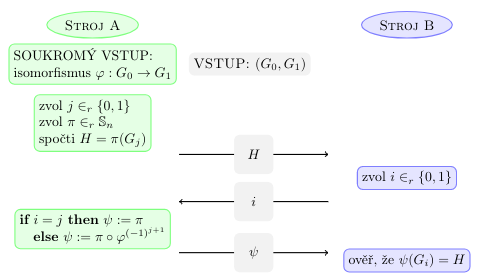
\includegraphics[width=0.5\linewidth]{graph_iso}
		\end{figure}

		Předpokládejme nyní, že $(G_0,G_1)\not\in GraphISO$, pak ale zpráva $H$ je, bez ohledu na postup $A^*$, isomorfní nejvýše jednomu z grafů. S pravděpodobností $1/2$ $B$ zvolí $i$, pro které neexistuje $\psi$ splňující $\phi(G_i)=H$. Ve dvou kolech tedy odmítne s pravděpodobností $3/4$ -- spolehlivost.

		Nyní je třeba dokázat nulovou znalost. $M$ může simulovat celý výpočet s výjimkou situace $\psi=\pi\circ\varphi^{-1}$, tj. $i \neq j$. S pr. $1/2$ (pr. volby $i \neq j$) simulace selže hned v prvním kole. Při dvou kolech je tato pravděpodobnost $1/4$ -- stačí tedy tři opakování pokusu o simulaci, aby se pravděpodobnost dostala nad $1/2$. $M$ tedy opakuje celý postup třikrát a vytiskne $\perp$, pokud všechny pokusy selhaly. Jinak vytiskne výstupní snímek $B^*$ po úspěšném pokusu.
	\end{proof}
\end{claim}

\subsection*{Hašovací funkce}
\begin{defn}[Hašovací funkce]
	Funkci $h:\{0,1\}^*\rightarrow\{0,1\}^n$ nazýváme hašovací funkcí. Obraz $h(x)$ nazýváme \textit{otisk}, \textit{hash} nebo \textit{digest} prvku $x$. Pro $x\neq y:h(x)=h(y)$ řekneme, že pár $(x,y)$ je kolize funkce $h$.
\end{defn}

\begin{defn}[Kryprografická hašovací funkce]
	Kryptografická hašovací funkce je hašovací funkce, která navíc splňuje 3 vlastnosti:
	\begin{itemize}
		\item \textbf{Preimage-resistance}: je obtížné nalézt $x$ pro dané $y$ t.ž. $h(x)=y$.
		\item \textbf{2nd-preimage-resistance}: je obtížné nalézt $x\neq x'$ pro dané $y$ t.ž. $h(x)=y=h(x')$.
		\item \textbf{Collision resistance} (bezkoliznost/kolizevzdornost): je obtížné nalézt $x,\,x'$ t.ž. $h(x)=h(x')$.
	\end{itemize}
\end{defn}

Formální definice může být zkonstruována například prostřednictvím zanedbatelné funkce. Nicméně v praxi má úskalí -- např. nevíme, zda-li existuje jednosměrná funkce, kterou bychom touto konstrukcí dostali.

Obecně máme dvě konstrukce pro hašovací funkce - Merkle-D$\mathring{\text{a}}$mgard (SHA1, SHA2, MD5) a houbovitá konstrukce (SHA3). Hlavní rozdíl mezi konstrukcemi je, že houbovité konstrukce ve výstupu nezveřejní svůj celý vnitřní stav. Toto například zabrání tzv. \textit{length-extension attack}.

\subsubsection*{Merkle-D$\mathring{\text{a}}$mgard}
Tato konstrukce má dvě varianty, které v praxi splývají. První varianta používá padding $x_n|10...0|length_{64}(x)$. Druhá varianta, která za cenu většího nafouknutí zprávy odstaní omezení na celkovou délku zprávy. Tato varianta prefixuje první blok $1$ a ostatní bloky $0$. Poslední blok je vyplněn stejným způsobem, jen místo délky zprávy se použije délka paddingu. Důkaz bezpečnosti pro obě varianty je velmi podobný, proto uvedeme důkaz pouze pro první variantu.

\begin{center}
	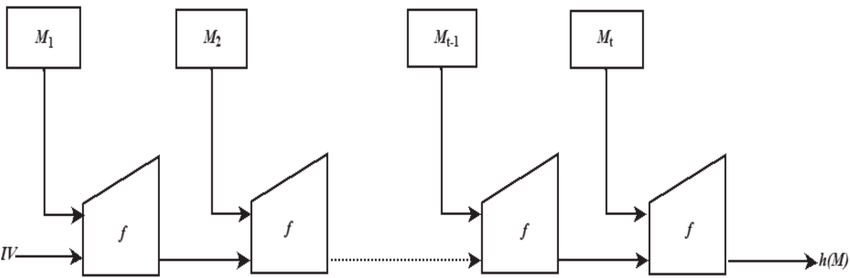
\includegraphics[width=0.5\linewidth]{MD.png}
\end{center}

\begin{thm}
	Je-li kompresní funkce $f:\{0,1\}^s\times\{0,1\}^b\rightarrow\{0,1\}^s$ kolizivzdorná, pak $h$ je též kolizivzdorná.
	\begin{proof}
		$x=B_1||\dots||B_n,x'=B'_1||\dots||B'_n$ t.ž. $h(x)=h(x'), x\neq x'$
		
		$\Rightarrow f(S_{n-1},B_n)=f(S'_{n-1},B'_n)$, tj, buď $(S_{n-1},B_n)\neq(S'_{n-1},B'_n)$ (a máme kolizi pro $f \Rightarrow$ spor nebo kolize nastala dříve. Jelikož $B_n$ a $B'_n$ obsahuje informaci o délce, pak jsou tyto zprávy $x$ a $x'$ stejně dlouhé.

		Indukčně postupujeme až k prvnímu bloku -- buďto nastala kolize v průběhu (což je spor s kolizivzdorností) nebo, jelikož první bloky musí být různé (dle předpokladu $x\neq x'$ a rovnosti $B_i=B'_i$ pro $i>1$ z indukčních kroků), nastala kolize v prvním bloku což je opět spor s kolizivzdorností $f$.
	\end{proof}
\end{thm}

\begin{rem}[Davies-Mayer schéma]
	Buď $E$ šifra, pak kompresní funkci dle Davies-Mayer schéma definujeme jako $f(S_{i-1},B_i)=E_{B_i}(S_{i-1})+S_{i-1}$, kde $+$ je celočíselné sčítání po slovech mod $2^{32}$. Tuto konstrukci používá mj. MD5, SHA-1, SHA-2.
\end{rem}

\subsubsection*{Houbovité konstrukce}
\begin{center}
	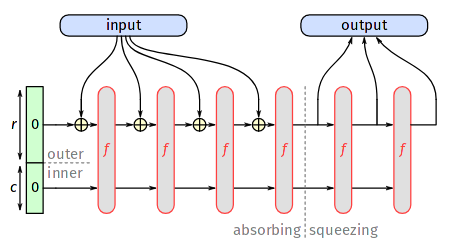
\includegraphics[width=\linewidth]{sponge.png}
\end{center}

Houbovité konstrukce mají dvě fáze -- absorpce a ždímání. Existují i konstrukce, které tyto fáze střídají (tzv. duplex), vstup

\begin{center}
	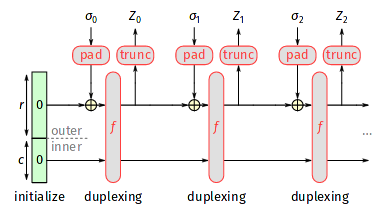
\includegraphics[width=\linewidth]{duplex.png}
\end{center}